\section{Konzept}

\subsection{Kontextdiagramm}
\begin{figure}[H]
  \begin{center}
    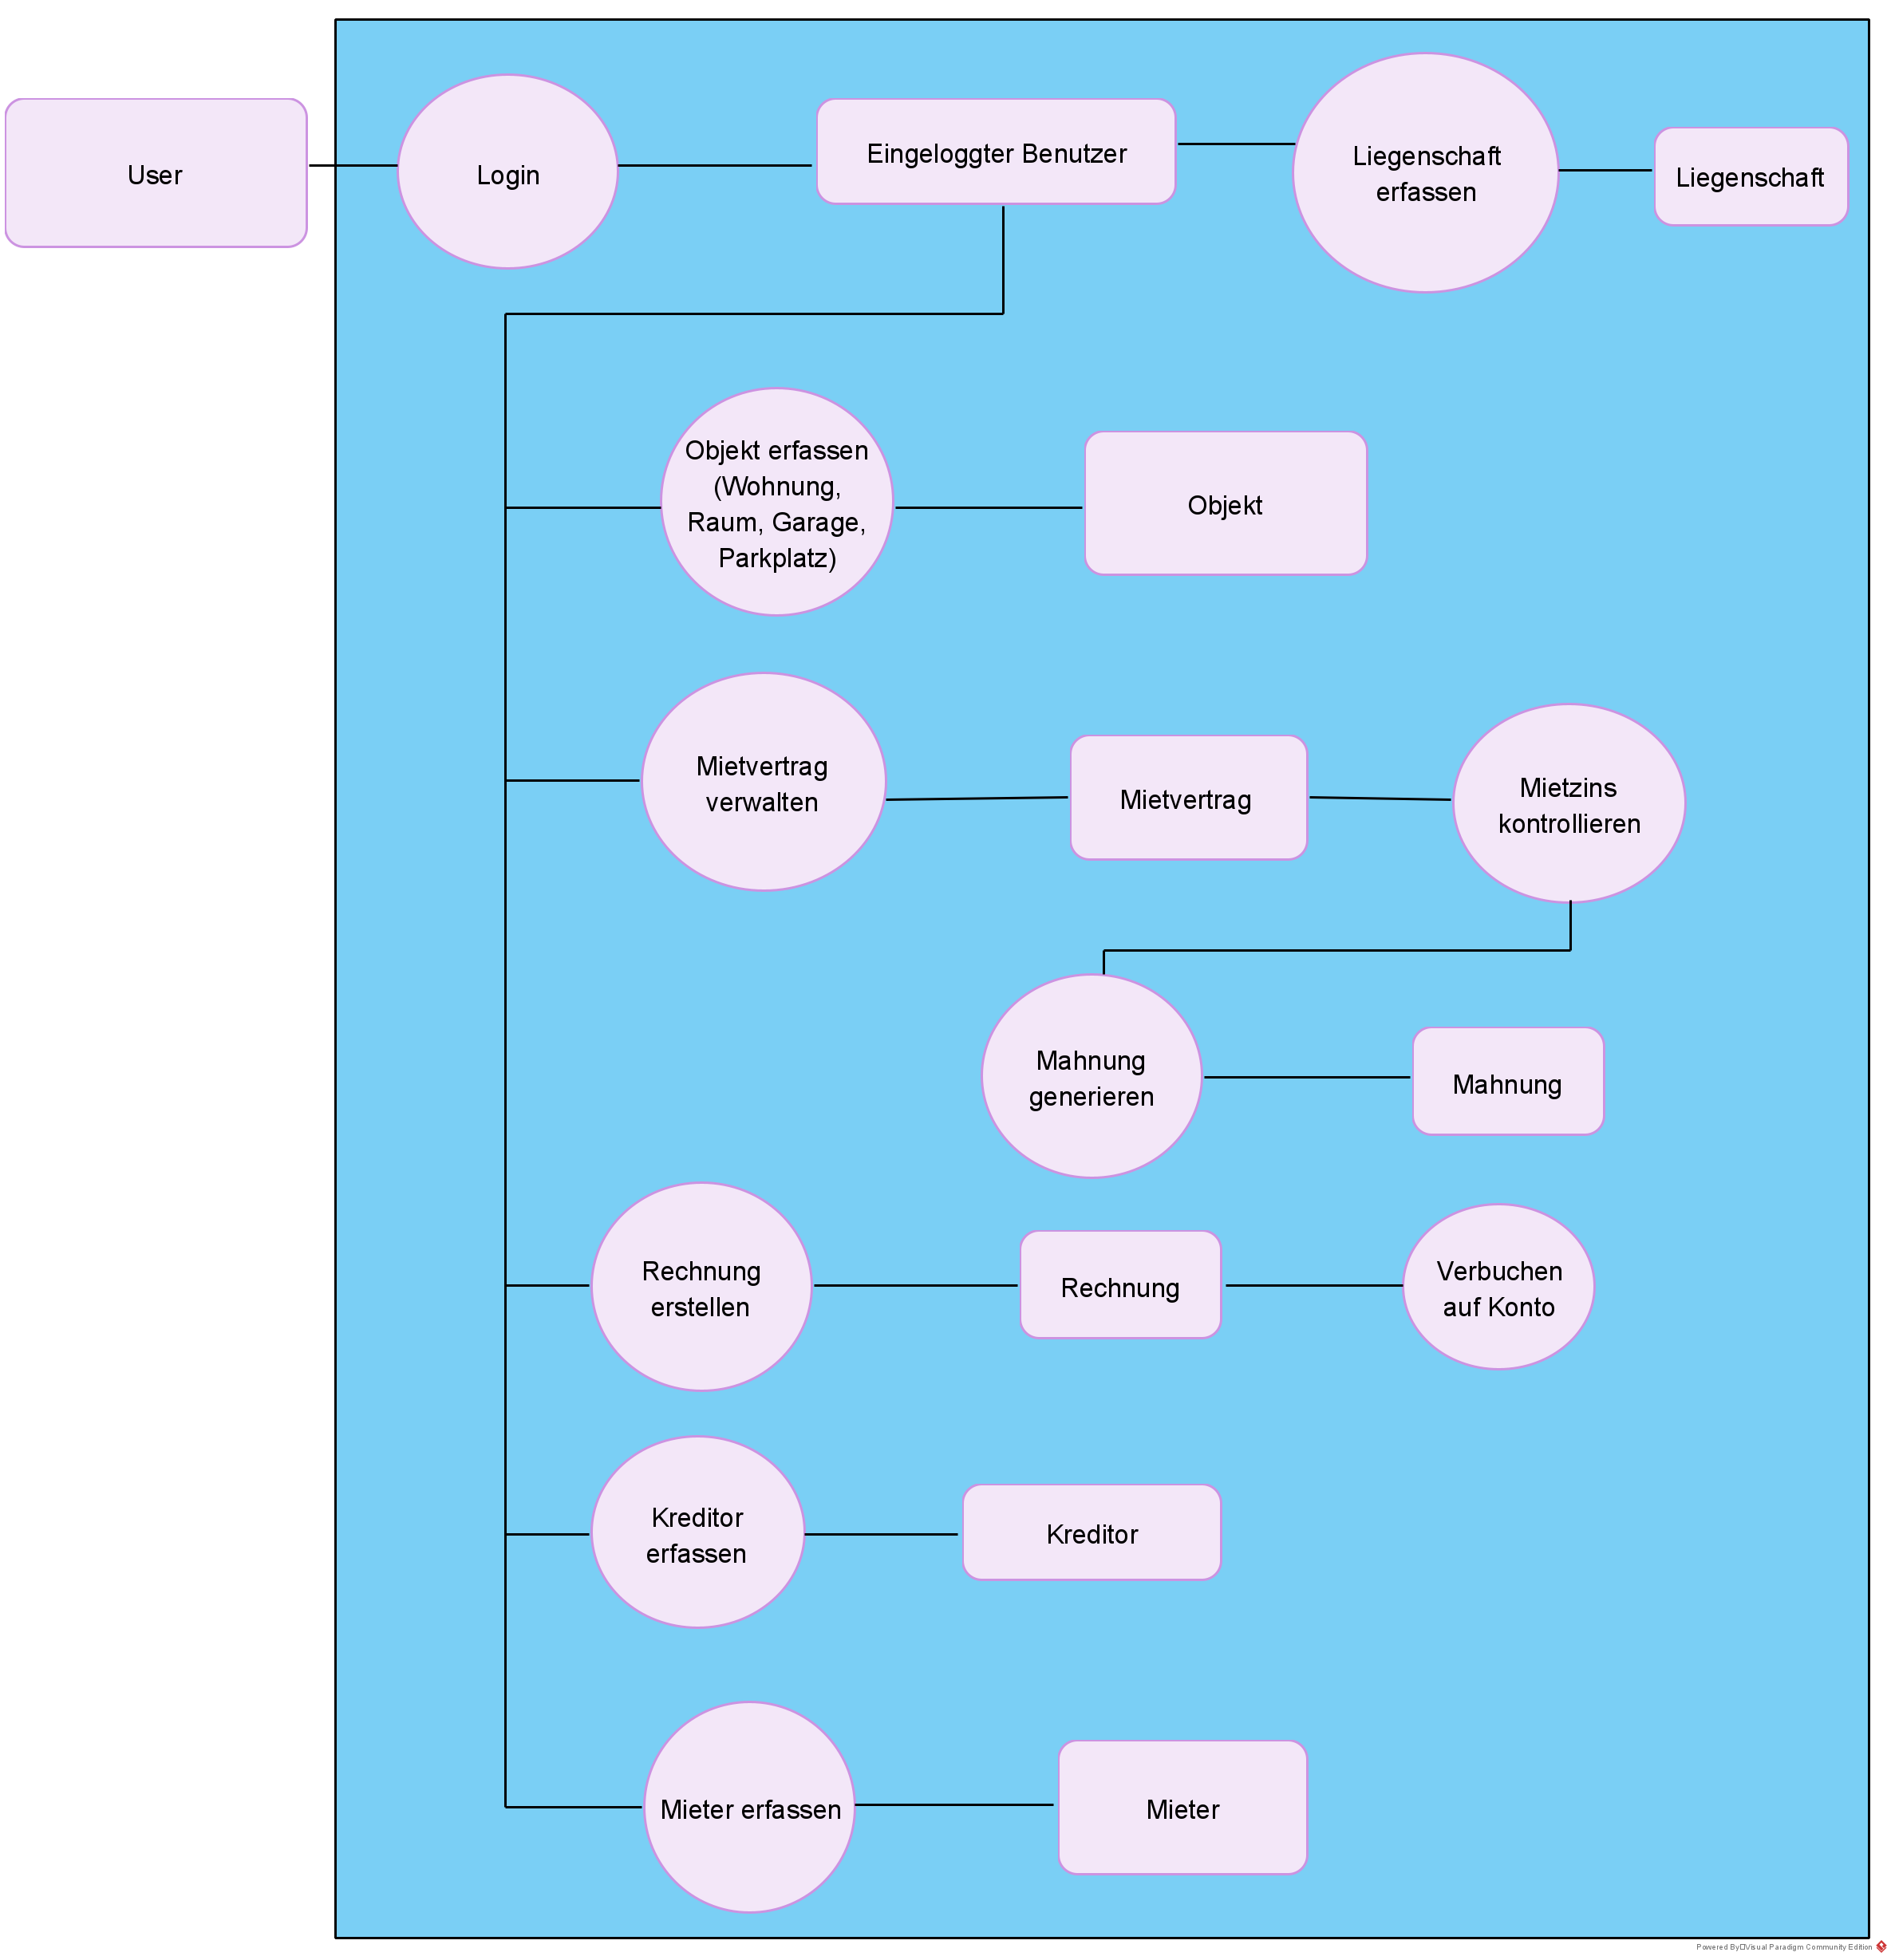
\includegraphics[width=0.99\linewidth]{content/diagrams/out/contextdiagram/context.png}
    \caption{Kontextdiagramm}
  \end{center}
\end{figure}

\subsection{Geschäftsprozessanalyse}
\subsection{Detailanforderungen an das neue System}

\subsection{Use-Case-Beschreibungen}
\subsection{Sequenzdiagramme}
\subsection{Modellierung der Klassen}
\begin{figure}[h]
  \begin{center}
    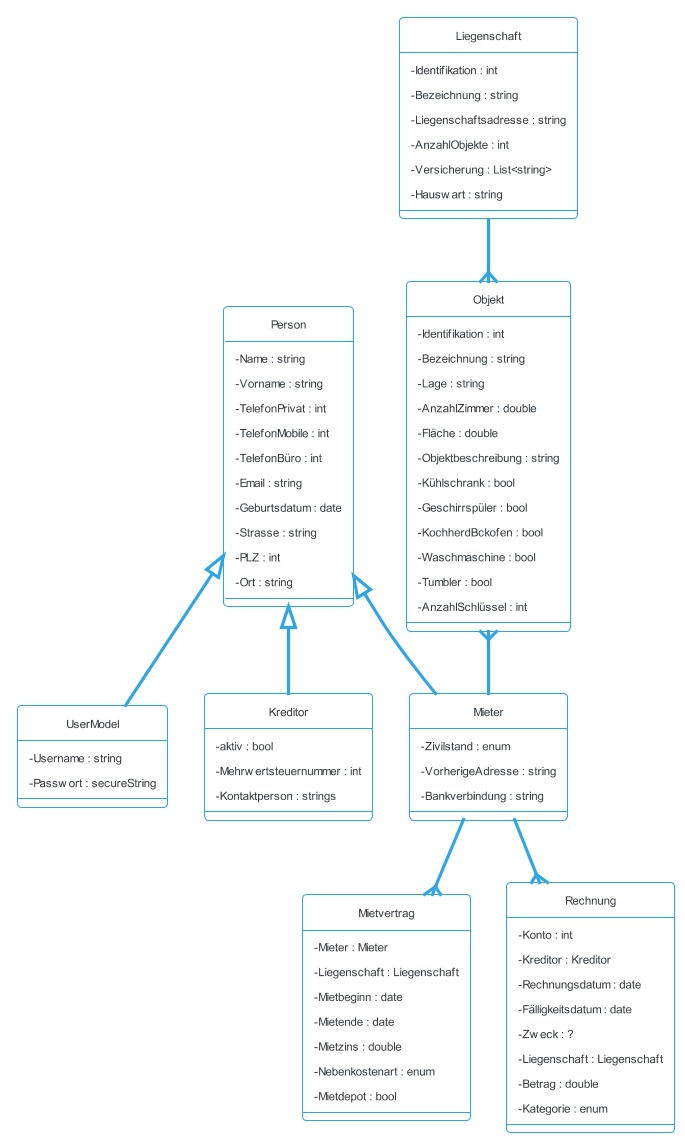
\includegraphics[width=0.75\linewidth]{content/diagrams/out/classdiagramm/ImmoGlobal.png}
    \caption{Klassendiagramm}
  \end{center}
\end{figure}

\subsection{Zustandsdiagramme}
\subsection{Modellierunge der Datenbank}
\subsubsection{ERD}
\subsubsection{Beschreibung der Fachentitäten, Beziehungen und der referenziellen Integritätsbedingungen}
\subsection{Systemarchitektur}
\subsection{Testkonzept}
\subsubsection{Vorgehen}
\subsubsection{Testobjekte}
\subsubsection{Testfälle}
\subsection{Einführungskonzept}
\subsection{GUI-Design}
